\chapter{Literature Review \label{sec:litReview}}


This chapter will explore and summarise previous work on the topic of passive bistatic radar detection and associated hardware, ranging from academic literature to currently available commercial technology. The literature review will be divided into the following sections: low cost IoT hardware receiver, digital signal based illuminator of opportunity and existing commercial technology.

\section{Low Cost IoT Hardware PBR Reciver Design \label{sec:lowCostIOT}}

The Swiss army have conduncted a very informative pilot study utilising both FM radio and DAB+ signals as illuminators of opportunity for an IoT based receiver design. Moser et. al explore the performance of a Raspberry PI 3 GPU and CPU against a quad-core intel i7 equipped PC \cite{IOTpassiveRadar}. This paper also provided a good starting point for information regarding the difference in signal processing between digital (DAB+) and analogue (FM) illuminators of opportunity, including key characteristics as seen in Figure \ref{fig:signals} . 

\begin{figure}[htbp]
    \centering
    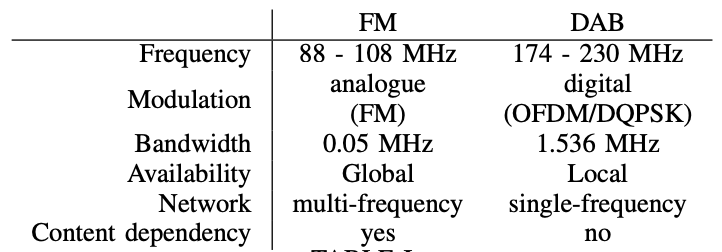
\includegraphics[width=0.4\textwidth]{digAnalog.png}
    \caption{Comparison Table - Analog vs Digital Signals \cite{IOTpassiveRadar}}
    \label{fig:signals}
\end{figure}

\par \vspace{0.5cm} 
\noindent Moser et. al also provide a summary of the range doppler map generation process which itself is derived from Batches algorithm \cite{DSPfm}, including valuable performance measurements which indicate the efficacy of GPU processing over CPU processing.  The specific hardware utilised in Moser's paper was a Raspberry Pi v3; 1.2GHz Cortex A53 CPU along with a 400MHz VideoCore IV GPU. As of writing, the estimated cost to recreate this exact hardware (including SDR-RTL hardware) would be approximately \$100 AUD, representing a very low cost setup. Noting that hardware has also made significant advancements since the time of the paper (2019), with the Raspberry Pi v5 now available. The paper provides good hardware reference values for real-time processing limits of DAB frame computations, a key consideration area when optimizing for low cost hardware, these comparisons can be viewed below \ref{fig:iotCompute}.

\begin{figure}[htbp]
    \centering
    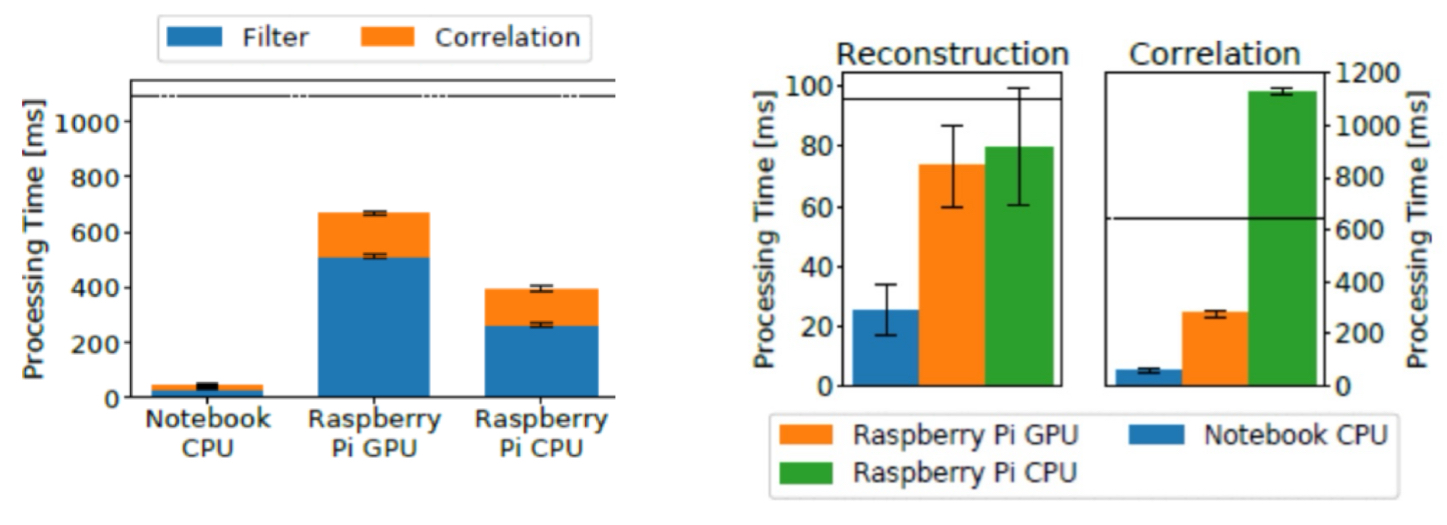
\includegraphics[width=0.5\textwidth]{moserHardware.jpeg}
    \caption{Hardware Compute Comparison with Real Tiem Reference \cite{IOTpassiveRadar}}
    \label{fig:iotCompute}
\end{figure}

Overall, this conference paper provides a good starting point for understanding the hardware requirements and limitations of a low cost IoT based passive bistatic radar receiver. Notably this paper is difference from the thesis proposed given that it focuses on implementing real time processing and optimisation of detection DSP algorithms on low cost hardware, rather than the design and construction of a user friendly, scaleable testbed, which also explores different SDR modules.

\section{Illuminators of Opportunity}

Throughout the literature review, a range of papers exploring illuminator signals were explored, the DTSO report Written by Palmer, Palumbo, Van Cao, and Howard provides a good theoretical basis. Whilst the scope of this proposal is confined to terrestrial illuminators (specifically digital audio), Palmer et. al highlight the wide range of use cases made available by other illuminators, including satellite signals and mobile phone signals. The report also provides a good overview of range doppler mapping, and target classification properties (despite the scope of this proposal not including target classification). Specifically, their is notable contrast of the utility of digital singals over analogue signals as demonstrated via the figures in \ref{sec:illuminators}, with the autocorrelation output of a terrestrial analogue TV broadcast shown to have poor IoO characteristics.

\begin{figure}[htbp]
    \centering
    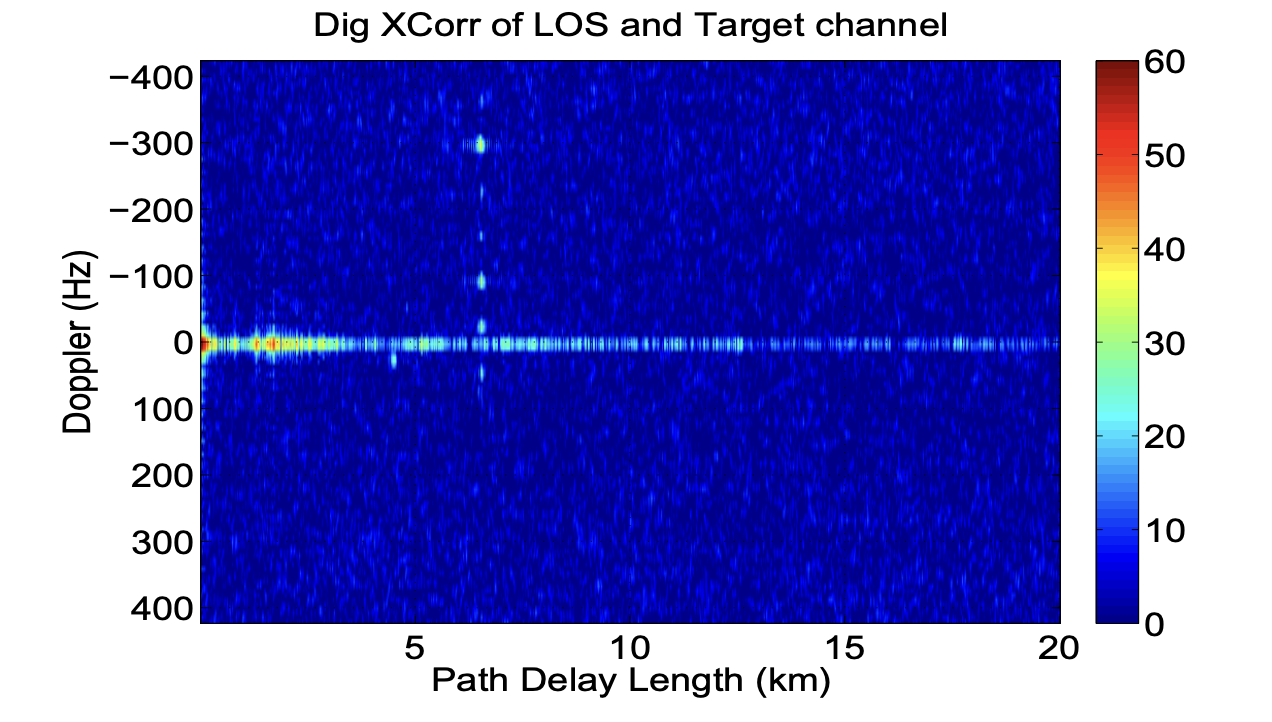
\includegraphics[width=0.7\textwidth]{movingTarget.jpg}
    \caption{RDM of target moving away from receiver \cite{DTSO2009}}
    \label{fig:rdm}
\end{figure}

\noindent As seen above in Figure \ref{fig:rdm}, in the .gif version of the image, the dot can be seen moving upwards (indicating motion away). This example also reflects effective de-cluttering of the RDM, a key step in passive tracking. An important consideration raised in this report is the edge case whereby the target moves along the bistatic ellipse as viewable in Figure \ref{fig: topology}, resulting in the doppler shift to be minimal and making tracking difficult.

Palmer et. al also effectively highlight the utility of thresholding and constant false alarm rate (CFAR) processing in the context of passive radar, with the CFAR algorithm being used to detect targets in the presence of clutter. CFAR represents a potential exploration area for this thesis in order to extend the effective detection range of a testbed via the differentiation of target and clutter signals.



\section{Existing Commercial Technology}
Commercial industry has been developing passive radar for a number of years now, with the majority of such development occuring in the military space. Specifically,these innovations are in the realm of air sureveillance and can be either ground based or air based \cite{FundamentalsPassiveRadar}. Structurally, passive radar provides numerous advantages for defence applications including covert tracking due to the lack of a transmitter.
\par \vspace{0.5cm} 
\noindent \textbf{Lockheed Martin - SilentSentry:} One of the earliest commercial products utilising passive radar, the SilentSentry utilises analog illuminator signals with a dual horizontal linear phased array antenna to passively detect and track airborne targets \cite{DTSO2009}. It claims a detection range of up to 200km with an azimuth coverage of 60-360 degrees. Given the analog nature of the signals (FM and other terrestrial signals), it has a receiver for the direct line of sight signal and the echoed target signal before applying a signal processing algorithm. The silent sentry also claims capability of detecting multiple targets simultaneously, a key feature for air surveillance applications \cite{SilentSentry}.

% Image of Silent Sentry
\begin{figure}[htbp]
    \centering
    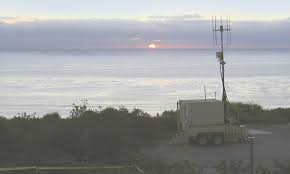
\includegraphics[width=0.4\textwidth]{silentSentry.jpeg}
    \caption{Silent Sentry Passive Radar \cite{SilentSentry}}
    \label{fig:silentSentry}
\end{figure}

Since the release of Silent Sentry in 1998, there have been a number of other releases from different countries, each utilising a combination of different illuminators. Notably, these systems include BAE Systems CELLDAR (UK), Thales Homelander Alerter (France), and Silentium Defence Maverick (Australia). 

\vspace{0.5cm}
In summary, the literature review has highlighted proof of concept, theory of illuminators and existing commercial technology. Importantly, this commercial technology comes with a large price tag, physical size and relatively large barriers to entry in terms of technical know-how. Moreover, the high end commercial systems are geared toward military grade tracking and detection. This thesis will aim to bridge the gap between demonstrated proof of concept and relatively simple theory to provide a low cost, user friendly testbed for passive radar detection. Subsequently enabling both hobbyist access and lower cost research and development in the field.